\chapter{Mycelium Machine \& Materials}


\section{Overview}

This projects aim to develop an easy way to make mycelium-based biocompisites. We present two similar Controlled Environment systems for mycelium based composite that can be developed easily with DIY and low cost hardware.
One of this project focus more on monitoring un data management, the other one is mare about modularity and transport 
In both cases, we're talking about controlled-environment systems with a closed space, thermal resistance or heating mats, temperature sensors, humidity modulators and associated relative humidity sensors, carbon dioxide sensors and fans for air renewal and circulation. 
And of course a control and data transmission system. 

% \begin{figure}[h]
%     \centering
%     \includegraphics{images/Myceliummachine.png}
%     \caption{System design representation}
%     \label{fig:}
% \end{figure} 

\section{Systems design}

The controlled Environment systems takes the form of a closed box, isolated from external climatic conditions. this box is where the inoculated substrate for mycelium growth is placed: “Mycelium grow space”. 
The Mycelium grow space is instrumented with climate sensors. in this case a relative humidity sensor, a temperature sensor and a carbon dioxide sensor. they are connected to an ESP-type microcontroller which handles data reading.
The ESP will then send the data via an MQTT protocol to a RaspberryPI acting as an MQTT broker and server for an Influx database. The data can then be visualized via a dashboard on a user's computer. 

On the ESP, a main user can select the desired climate variables. This will change the conditions according to which the microcontroller will activate or deactivate relays. This will switch on or off climatic actuators (ie: thermal resistance etc...) which will also change the internal climatic conditions in the space.  
Everything will act automatically once the variables have been chosen by the user (Automation loop). 

This architecture allows the simultaneous use of several controlled environments with different growth conditions. Users can choose, via the MQTT protocol, whether or not to subscribe to a controlled environment and see the data associated with it. 

\begin{figure}[h]
    \centering
    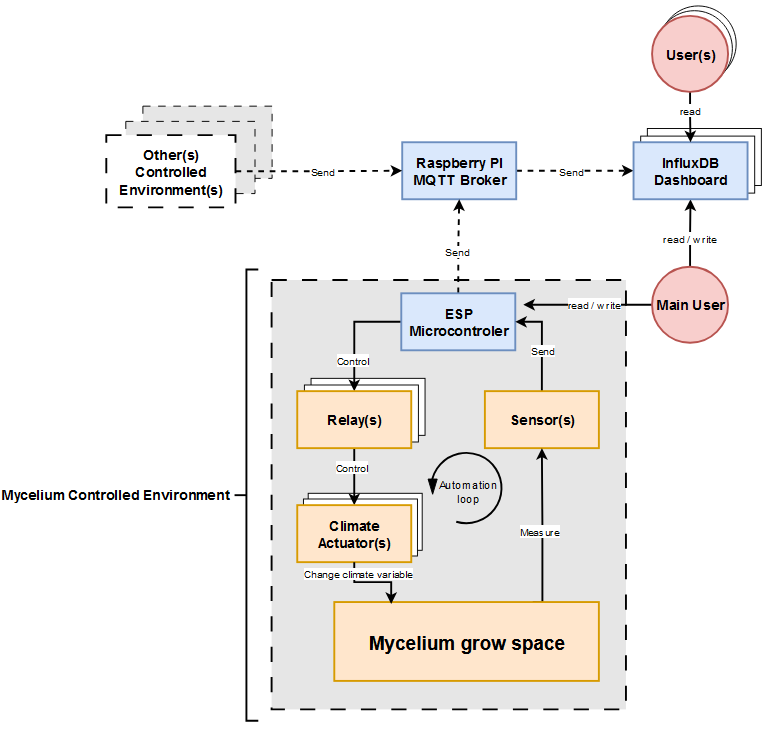
\includegraphics[width=1.4\textwidth]{images/diagMyceliummachine2.png}
    \caption{System design representation}
    \label{fig:blasttrash}
\end{figure} 


\section{Manufacturing Processes \& Grow Theory}

In a natural environment, the mycelium grows in the soil in search of nutrients. when it emerges from the soil into the air or under leaves, it is still in an environment rich in carbon dioxide. at this point, the mushroom stem (fruit of the mycelium) will grow until it reaches the air with more oxygen and forms the mushroom cap. 

In the case of Mycelium-based biocomposite, the mycelium will be innoculated in a substrate rich in nutrients and/or fibrous material. 

As explained above, the mycelium will agglomerate the substrate, greatly increasing the solidity of the innoculated substrate compared with the solidity prior to growth. 
When the mycelium comes into contact with the substrate in an oxygen-rich environment, it will blach and form a hydrophobic, fireproof layer.
That is why control carbon dioxide concentration is very important for mycelium material

Air renewal is also important for two other reasons: on the one hand, mushrooms breathe like we do, so they consume oxygen and spit out carbon dioxide. So the carbon dioxide concentration in the closed enclosure increases over time. Without air renewal, the mycelium will eventually aphyxiate itself. 
On the other hand, air renewal reduces the appearance and development of other pathogens or molds that would compete with the mycelium, and thus reduce its development. 


\paragraph[short]{Manufacturin Processes}

The approach is very similar to the literature described above \ref{Fab_process}.
first, the substrate is sterilized. then mycelium is mixed with the substrate in molds and placed in the controlled Environment for two or three weeks. 

During growth, once the mycelium has grown enough that the inoculated substrate no longer needs to be in the mold for growth. 
Then the molds are carefully removed to allow the mycelium to breathe as much as possible, especially on the surfaces in contact with the mold. 

After the growing phase, the Mycelium based biocompisites are dried in an oven for a minimum of 5 hours, depending on size or thickness, at a maximum of 80°C. 

\section{Contribution}

\subsection{Environment controlled}

The project consists of 3 main sections: the mycelium growth area, the water tank and the electrical panel.

The mycelium-growing part is a plastic box of around 100 liters, with its walls lined with bubble-wrap to provide thermal and light insulation. The box has also been modified by adding elastics to create tiers in the box to accommodate the molds and ensure uniform air circulation. The box houses the sensors directly connected to the electric panel and also houses thermal resistance. This section has 3 pipes. 2 for the air inlet and outlet sent by the filter fans, and one connected to the water tank.

The water tank consists of a water box containing a fogger and a centrifugal fan, both of which are connected to the electrical panel. There is an air inlet and an air outlet. The fan is located at the air inlet, while the air outlet is connected by a pipe to the growth space.

The fogger is immersed in the water in the reservoir. When the fogger and fan are switched on, the fogger will create an aerosol of water which will be transported to the growth space via the air flow created by the fan. This will increase the humidity in the growth space.

The electrical panel manages all the electrical or electronic parts of the project. In other words, the power supply, the microcontroller and the relays that control the various climatic actuators. The electrical panel is connected via a mains socket to power the entire system.

Everything was placed on a large board overlaid with wheels for ease of movement. 

\begin{figure}[h]
    \centering
    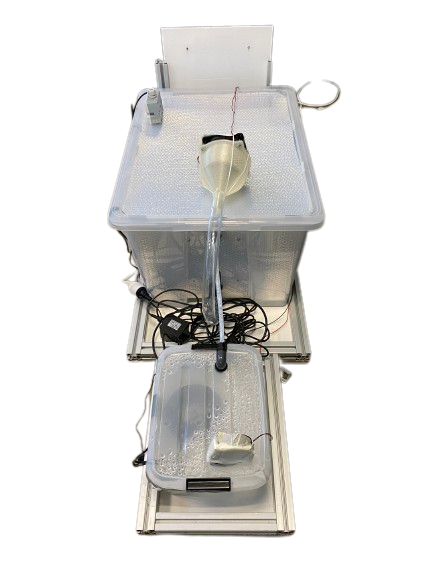
\includegraphics{images/myceliummachine.png}
    \caption{Environment controlled for mycelium picture}
    \label{fig:Mycemachinne}
\end{figure} 


The mycelium used was ganoderma lucidum, also known as reishi, the most widely used mushroom in the literature.\cite{yang2021material}
Moreover, this mushroom seems to have better mechanical properties, even if it seems that it's mainly the subtrate that dominates over the mechanical properties. 

Several types of substrate have been tested. More fibrous substrates such as coconut fiber. More granular substrates such as corn husks. Nutrient-rich substrates such as coffee grounds. Low-organic substrates composed mainly of minerals. 
And combination mixes of its substrates.

In addition, the direction of the fibers in the substrate also affects the mechanical properties. In other word fibrous substrates may have greater mechanical properties or the opposite, depending on how they were placed in the substrate.

\paragraph{Software}
There are 2 programs for the project. the program on the esp that reads the data, activates or deactivates the relays, and sends the data to the servers on the rasberry. 
And the program on the raspberry which receives the data and displays it via a dashboard in an influxDB database. 

On the ESP, the main user chooses the climatic variables for activating and deactivating the climatic actuator. In other words, the user chooses the climatic variables in which the system will be located. For example, for relative humidity, if the user chooses that the environment to be controlled should be between 80\% and 90\% humidity. Then when the humidity sensor reads that the humidity is below 80\%, ESP will activate (via the relays) the climatic actuators responsible for humidity control, i.e. the fogger and fan. Afterwards, ESP will deactivate the actuators once the sensor returns a humidity above 90\%.

It will be the same for the control of other climatic variables. 

In pallalele, the data read by the sensors will be sent via MQTT to an influx database on hermger on a raspberry. 
Influxdb is a database management system. in particular, it can be used to create dashboards, which can be used to monitor sensor data directly from a computer connected to the database. 

\begin{figure}[h]
    \centering
    \includegraphics{images/laptopdashboard.png}
    \caption{dashboard of mycelium controlled environent}
    \label{fig:Mycemachinne}
\end{figure} 

\paragraph{hardware}

\subsection{Modular environmental control}

This design is quite different from the contolled environment presented just before. 
The aim here is to present an easy way of unpacking a controlled environment. Firstly, the system can be completely dismantled to take up as little space as possible. 

The 3 sections presented above (I.e : the mycelium growth area, the water tank and the electrical panel.) are also found in this system to perform the same functions, but they have different characteristics.

The mycelium growth area,consists of a parallelepiped formed by aluminum profiles for the edges and cushions made from 2 sheets of transparent PVC for the faces. The cushions are inflated with air to provide better thermal insulation. These faces are fixed to the aluminum profile via velco tape. The top and bottom faces (the smallest faces) are in plexiglass. 

This is the part that takes up the most space in traditional designs. Here, all the growth  space is removable. The PVC sides can be deflated and then folded. The aluminum profiles can be removed to take up less space.

The equivalent of the electrical panel is located under the growth space in a small space in an MDF box where the electronics and power supply are located. There are several cables running in and out of this section the main power cable and the power supplies for the sensors and climatic actuators except for the fogger. Inside this hole are the relays and the microcontroller. 

The second special feature of this system is that the water reservoir and the fogger are not located close to the system, but are connected to it by a pipe. The water reservoir constantly generates water aerosol, and humidity is supplied via a fan in the growth space. 
Which makes it easy to centralize several contrasting environments around the tank for testing different cliamatic variables at the same time. 

%%%%%% photo avant apres demontage 
photo avant apres demontage ???????









\section{Result}


\begin{figure}[h]
    \centering
    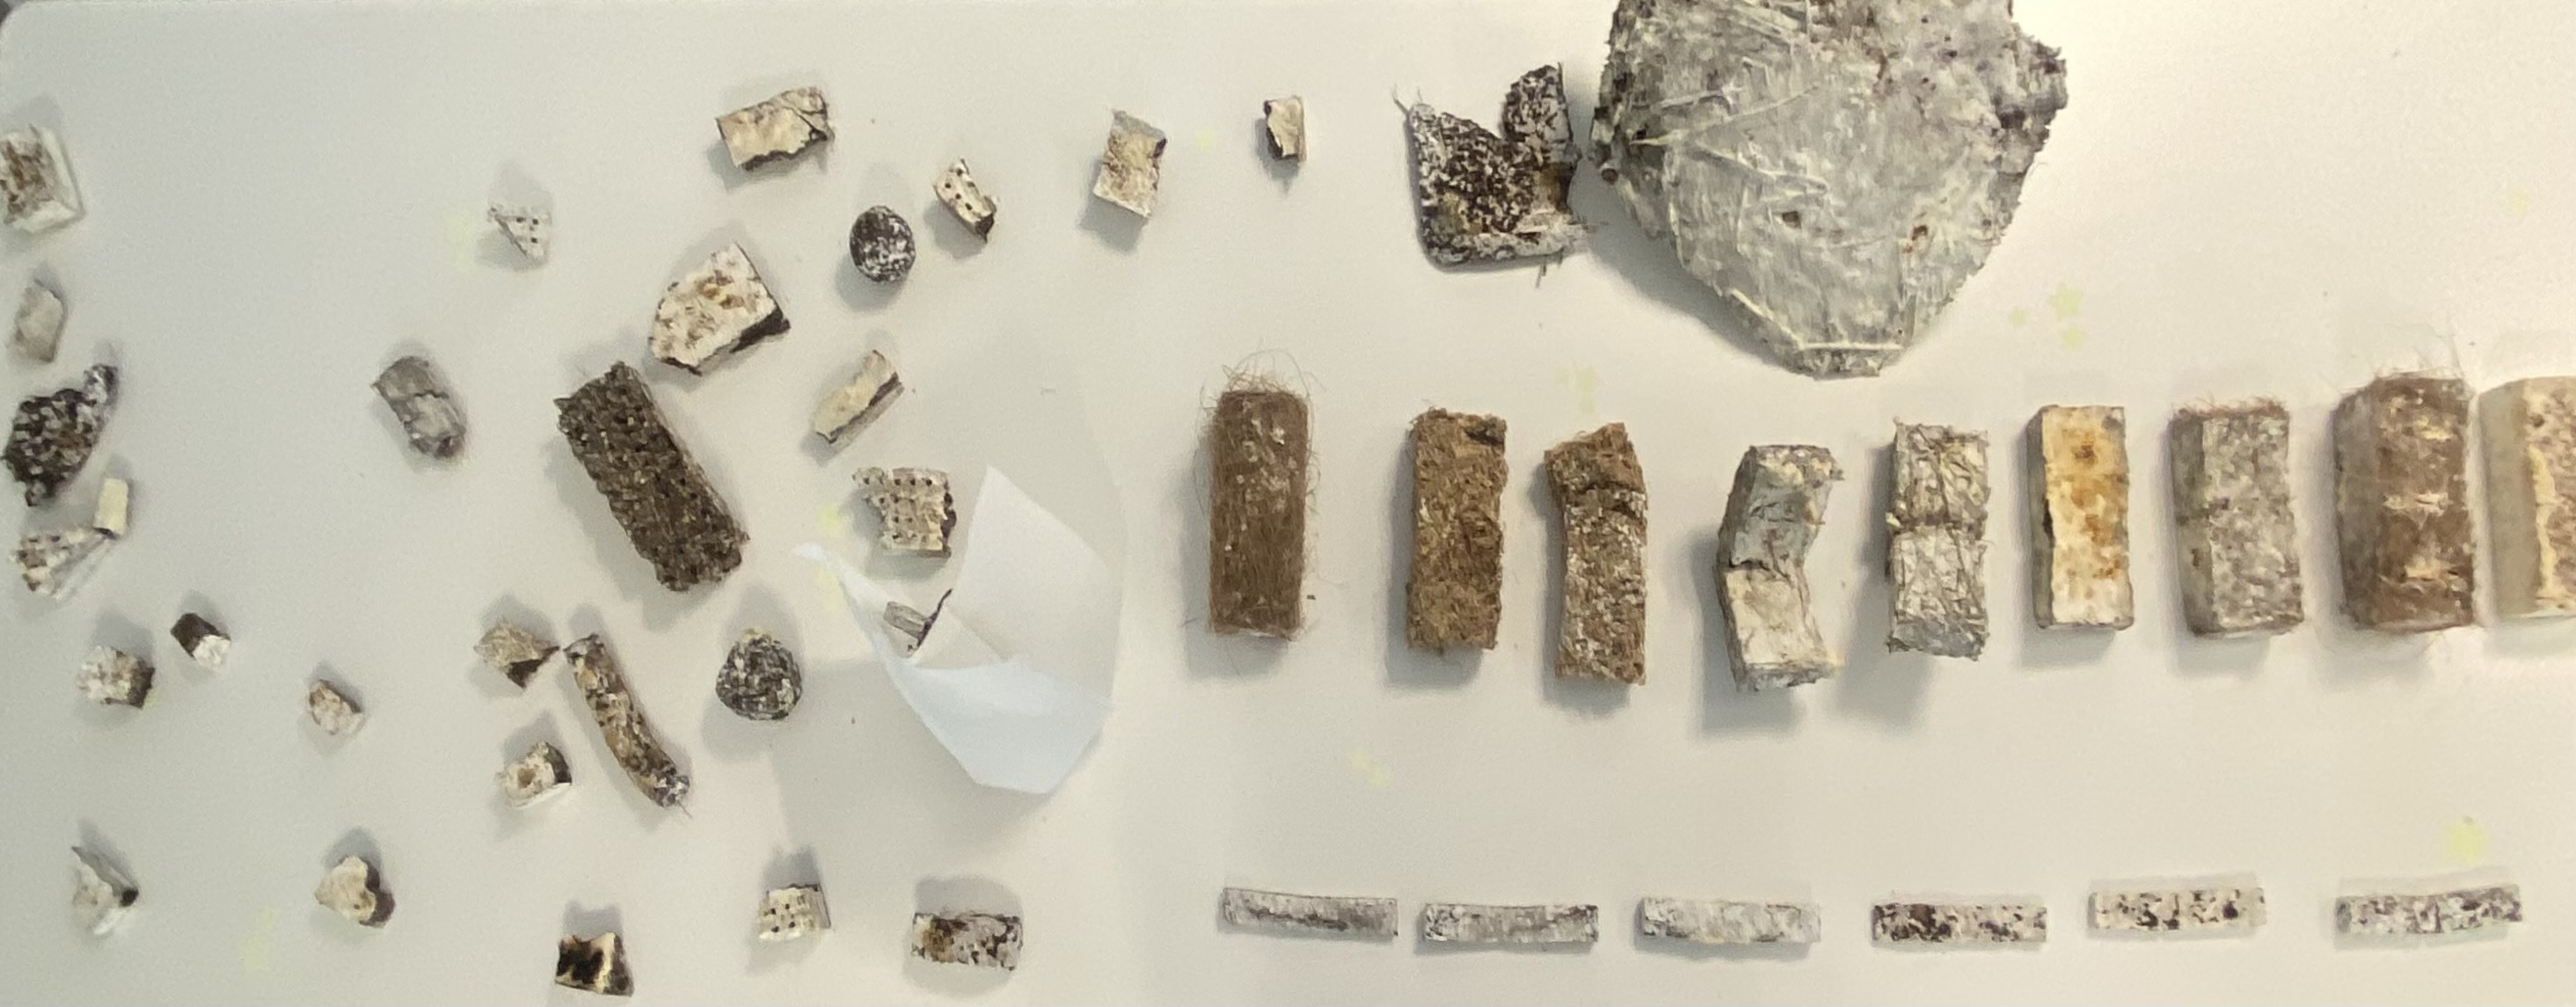
\includegraphics{images/resultMyce.png}
    \caption{Mycelium based materials with different substate}
    \label{fig:Mycemachinne}
\end{figure} 


\subsection{Mechanical test}


